El fotomultiplicador de Silicio es un dispositivo de detección de radiación relativamente nuevo en el mercado que surge como alternativa al tubo fotomultiplicador. Este consiste en un array bidimensional formado por multiples pixels independientes y alimentados en paralelo (mismo voltaje operacional para cada uno) a un voltaje tal que les permita estar en modo Geiger. Cada uno de los pixels actua como un APD (fotodiodos de avalancha).

Cuando detectan un foton estos pixels producen una cascada de pares electrón hueco que pasará a formar parte de la señal del sistema de detección, la cual estará formada por la suma de las señales de cada pixel que han detectado un fotón para cada instante de tiempo. Idealmente cada pixel únicamente puede detectar un fotón. Dado que poseen una alta eficiencia de fotodetección los SiPM son utilizados como contadores de fotones, especialmente para señales débiles.

Debido a ello presenta una serie de propiedades distintas a los convencionales tubos fotomultiplicadores que lo hacen ideal para unas situaciones y no tanto para otras, como por ejemplo su tamaño compacto, inmunidad a campos magnéticos, electrónica sencilla, alta eficiencia de detección de fotones (especialmente adecuado para nuestro experimento), buena linealidad, dependencia con la temperatura, alta ganancia a menor voltaje de alimentación y, por extensión, menor consumo, tiempo de respuesta corto y, por extensión, buena resolución temporal.

Hay que tener en cuenta que los SiPM son detectores de estado sólido y, por extensión, presentan ruido térmico, ruido que se verá amplificado por el hecho de estar operando en modo Geiger. Este ruido es denominado corriente oscura (Dark counts) y su forma se ve reflejada en la siguiente figura:

\begin{figure}[hbtp]
\centering
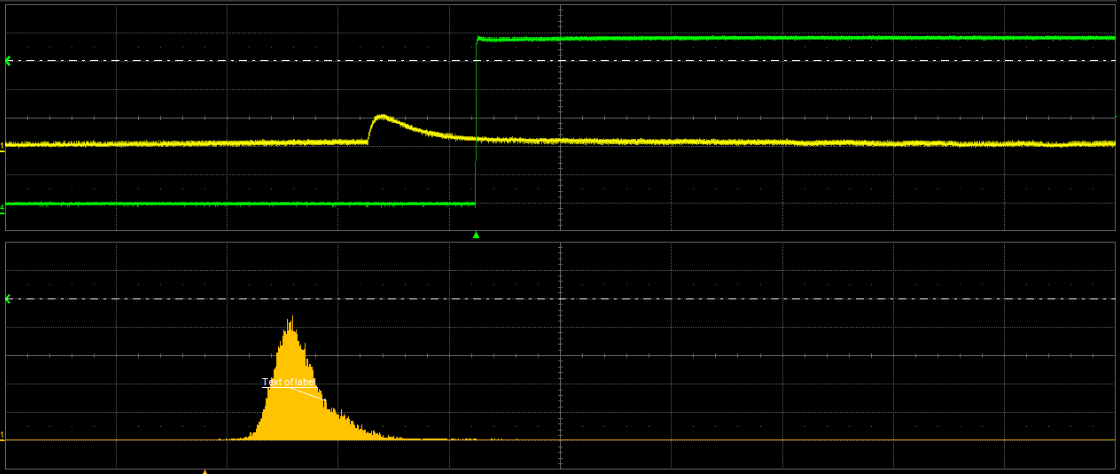
\includegraphics[scale=0.2]{pedestal.png}
\caption{\textbf{Figura 2}.- Dark counts}
\end{figure}

Cuando trabajemos con detectores de estado sólido debemos trabajar en condiciones de voltaje operacional y temperatura óptimas para poder medir con el detector ya  que, estas cuentas oscuras dependen de estas magnitudes y pueden llegar a ser tan numerosas que absorban por completo la señal del sistema. También podemos reducir su importancia sobre la medida con ayuda de triggers, por ejemplo, medir únicamente cuando la señal de entrada del sistema este activa (si se conoce este intervalo de tiempo). En cualquier caso siempre se deberá realizar una medida del pedestal (sin señal de entrada) para tener en cuenta el número y características de los eventos que van a contribuir a la señal sin proceder de la misma y utilizar esta información para el posterior análisis. 

En esta sección nos proponemos desarrollar un método de compensación para las variaciones de la ganancia de un fotomultiplicador de silicio derivadas de la temperatura a partir de variaciones derivadas del voltaje de alimentación del SiPM (voltaje de desertización), de ahora en adelante llamado voltaje operacional. 

En concreto utilizaremos el modelo S13360-1375CS de hamamatsu, ya que será el modelo que utilizaremos en el prototipo del experimento. Se ha elegido este modelo ya que presenta una eficiencia de fotodetección máxima entorno a los $450~\nm$, que corresponde aproximadamente a la longitud de onda del azul, $435~\nm$ y, en concreto, se asemeja bastante con el máximo de la energía reemitida por las fibras centelleadoras BCF-12, $435~\nm$, encargadas de detectar la radiación $\beta$ del agua tritiada en nuestro experimento como puede apreciarse en la siguiente figura. Con esto conseguiremos que la señal sea tan grande como sea posible, algo fundamental ya que, como ya se ha mencionado, una de las principales dificultados del experimento es que estamos intentando extraer una señal muy pequeña.

\begin{figure}[htb]
\centering
{
%\subfloat[PDE]
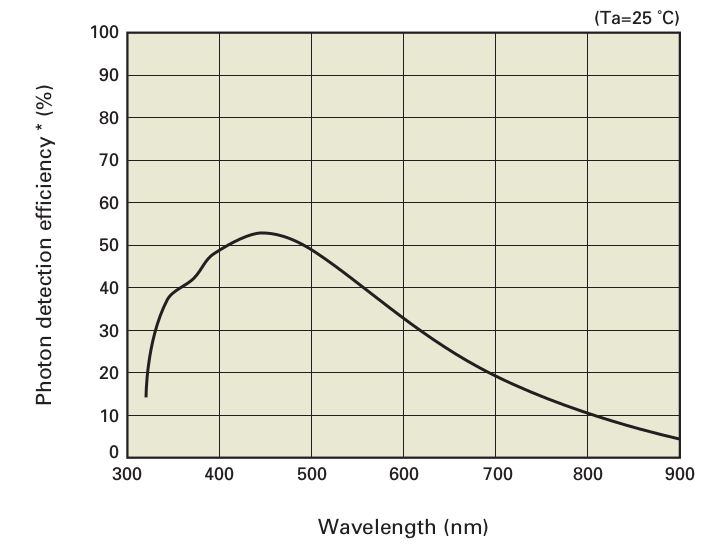
\includegraphics[scale=0.3]{PED.png} 
}
{
%\subfloat[Espectro de emisión]
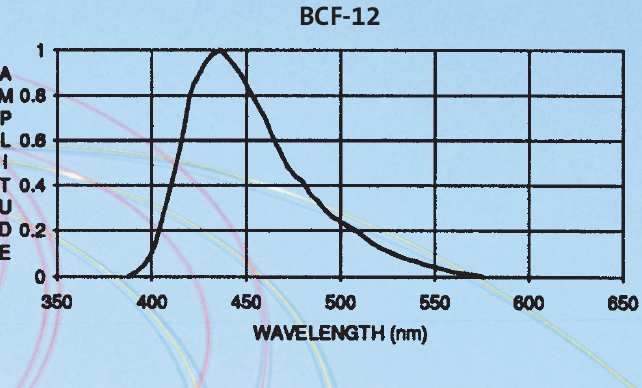
\includegraphics[scale=0.35]{EmisionBCF12.png} 
}
\caption{\textbf{Figura 3}.-PDE del SiPM y espectro de emisión de las fibras respectivamente}
\end{figure}

La forma de abordar este método de compensación de la ganancia ha sido el siguiente:
\begin{enumerate}
\item {} 
Por un lado se ha realizado una calibración de la ganancia frente a la temperatura obteniendo su relación de dependencia. Para ello se ha necesitado la utilización de un sistema de control de temperatura. En concreto se ha utilizado un sistema de la marca DYCOMETAL, (modelo CCM 81) que permite controlar temperatura y humedad relativa con una precisión de $0.1$ grados  y  $0.5$\% respectivamente.

\item {} Por otro lado se ha realizado una calibración de la ganancia frente al voltaje operacional obteniendo su relación de dependencia. Para obtener este voltaje operacional se ha utilizado un electrómetro de la marca KEITHLEY, en concreto el modelo 6517B, el cual presenta una resolución inferior al mV, más que suficiente para considerar este totalmente constante ya que se necesitan mayores modificaciones para que estas sean apreciables en la ganancia.

\item {} Finalmente, a partir de estas dos dependencias determiandas, se ha obtenido la ecuación de dependencia entre voltaje operacional y temperatura que nos determine una ganancia constante  y se ha realizado un test de comprobación para esta relación.
\end{enumerate}

El objetivo final de este estudio será mantener la ganancia del fotomultiplicador de silicio constante ante variaciones involuntarias de la temperatura a partir de variaciones voluntarias con el voltaje operacional. Esta es una correción fundamental para el objetivo final del detector ya que de lo contrario (no) obtendríamos alertas de fugas de tritio cuando estas no (si) han ocurrido, cuando, en realidad, lo único que ha ocurrido ha sido una modificación de temperatura.